\Chapter{Trabajo y Resultados}{Implementación, Optimización, Experimentos y Resultados}

\section{Implementación}
\index{Implementación A*}

Tanto \Python como C++ son lenguajes orientados a objetos.
Esta sección contiene las descripciones de las diferentes
clases diseñadas para dar soporte al algoritmo.

\begin{notebox}
El principal contenido de esta investigación es el estudio
de distintas implementaciones paralelas del algoritmo A*,
por ello es necesario tener alguna noción sobre la Implementación
del algoritmo.
\end{notebox}

\subsection{Task}
\index{Implementación A*!Task}

La clase \lstinline{Task} correspone a una tarea a realizar.
Una instancia de esta clase está definida por los atributos:
\begin{itemize}[itemsep=0.25px]
    \item \lstinline{unsigned int duration}: Duración de la tarea.
    \item \lstinline{std::vector<int> qualified_workers}: Listado de trabajadores que pueden realizar la tarea.
\end{itemize}

\subsection{State}
\index{Implementación A*!State}

La clase \lstinline{State} corresponde a un estado (o nodo).
Una instancia de esta clase está definida por los atributos:
\begin{itemize}[itemsep=0.25px]
    \item \lstinline{std::vector<std::vector<Task>> jobs}: Lista de trabajos y tareas a ejecutar.
    \item \lstinline{std::vector<std::vector<int>> schedule}: Planificación actual.
    \item \lstinline{std::vector<int> workers_status}: Instantes en los que cada trabajador queda libre.
\end{itemize}

\begin{notebox}
    Nótese que el atributo \lstinline{std::vector<std::vector<Task>> jobs} será el mismo
    en todos los estados de un mismo problema.
    Por lo que no será necesario revisarlo en
    \lstinline{State::operator==} ni \lstinline{State::operator()}.
    Si el consumo de memoria fuese de importancia,
    sería posible utilizar una referencia para evitar
    almacenar esta estructura múltiples veces.
\end{notebox}

El algoritmo A* requiere que se creen estructuras de datos que contendrán instancias
de la clase \lstinline{State}.
Estas estructuras necesitan que se proporcionen implementaciones para los operadores
\lstinline{State::operator==} y \lstinline{State::operator()} de la clase \lstinline{State}.
Para diseñar las implementaciones de estos operadores
se estudian previamente los atributos que componen la clase \lstinline{State}:

\begin{itemize}[itemsep=0.25px]
    \item \lstinline{std::vector<std::vector<Task>> jobs}: Es igual en todas las
    instancias de \lstinline{State}, por lo que será ignorado.
    \item \lstinline{std::vector<std::vector<int>> schedule}: Proporciona
    información crucial sobre el estado ($cost_g$ y $cost_h$).
    \item \lstinline{std::vector<int> workers_status}: No proporciona
    información alguna sobre los costes,
    pero es necesario para distinguir dos estados diferentes
    ya que es posible que dos estados tengan los mismos costes pero a través de
    planificaciones distintas.
\end{itemize}

Por ello, será necesario definir dos operadores \lstinline{State::operator()}:
uno que sea indiferente al atributo \lstinline{std::vector<int> workers_status}
(\lstinline{StateHash::operator()})
y otro que sí lo tenga en cuenta para distinguir diferentes instancias de \lstinline{State}
(\lstinline{FullHash::operator()}).

\pagebreak
\section{Optimización}
\index{Optimización A*}

\subsection{Algoritmo A* monohilo}
\index{Optimización A*!Monohilo}

La siguiente subsección estudia la optimización
del algoritmo A* sin tener en cuenta el paralelismo,
esto es, se trata de optimizar el rendimiento
monohilo del mismo.

\subsubsection{State}
\index{Optimización A*!Monohilo!State}

La operación \lstinline{operator()} es ejecutada varias veces para cada
\lstinline{State}, este método tiene una complejidad de $O(n^2)$,
por lo que su valor se almacena tras calcularlo por primera vez
en un atributo del propio \lstinline{State}.

Los operadores \lstinline{operator==} necesarios se implementan utilizando
los \lstinline{operator()} correspondientes.
Las funciones hash utilizadas en los \lstinline{operator()}
son resistentes a colisiones,
esto es, $
h(State_a) \ne h(State_b) \iff State_a \ne State_b
$
por lo que se pueden
utilizar para comparar elementos en \lstinline{operator==}.

\pagebreak
\subsubsection{Coste H - Heurístico}
\index{Optimización A*!Monohilo!Heurísticos}
\label{ssec:Heuristicos}

La principal decisión que afectará al tiempo de ejecución
del algoritmo se encuentra en la Implementación
de la función heurística encargada de calcular el coste H.
Este coste se utiliza para seleccionar el siguiente nodo
a expandir, por lo que un buen heurístico es aquel que
mejor dirige al algoritmo en la dirección del nodo objetivo.

El rendimiento y calidad del resultado del algoritmo
dependerán en gran medida de la función seleccionada.
En algunos casos la implementación retornará resultados
óptimos (o cercanos al óptimo) pero requerirá un mayor tiempo
de ejecución, mientras que otras implementaciones
requerirán un menor tiempo de ejecución pero sus resultados
no serán óptimos.
Dependiendo del problema a resolver será conveniente implementar
una función heurística de un tipo u otro.

\paragraph{Heurístico para optimalidad}~
\index{Optimización A*!Monohilo!Heurísticos!Resultado Óptimo}

La siguiente implementación de la función heurística
dirigirá al algoritmo hacia nodos solución que sean óptimos
o se encuentren relativamente cerca del óptimo.

\begin{lstlisting}[language=C++]
unsigned int State::calculate_h_cost() const
{
    std::vector<int> h_costs;
    for (size_t job_idx = 0; job_idx < this->m_jobs.size(); job_idx++)
    {
        h_costs.emplace_back(0);
        std::vector<Task> job = this->m_jobs[job_idx];
        for (size_t task_idx = 0; task_idx < job.size(); task_idx++)
            if (this->get_schedule()[job_idx][task_idx] == -1)
                h_costs[job_idx] += job[task_idx].get_duration();
    }
    auto max_element = std::max_element(h_costs.begin(), h_costs.end());
    return max_element == h_costs.end() ? 0 : *max_element;
}
\end{lstlisting}

La función calcula el tiempo necesario para completar cada trabajo
y retorna el tiempo mayor.

\pagebreak

\paragraph{Heurístico para tiempo}~
\index{Optimización A*!Monohilo!Heurísticos!Rápido}

La siguiente implementación de la función heurística
dirigirá al algoritmo hacia cualquier nodo solución
independientemente de si es óptimo o no.

\begin{lstlisting}[language=C++]
unsigned int State::calculate_h_cost() const
{
    unsigned int unscheduled_tasks_count = 0;
    for (std::size_t job_idx = 0; job_idx < this->m_jobs.size(); job_idx++)
        for (std::size_t task_idx = 0; task_idx < this->m_jobs[job_idx].size(); task_idx++)
            if (this->m_schedule[job_idx][task_idx] == -1)
                unscheduled_tasks_count += this->m_jobs[job_idx][task_idx].get_duration();
    return unscheduled_tasks_count; 
}
\end{lstlisting}

La función calcula el tiempo necesario para completar
las tareas restantes si se ejecutasen una a una
y retorna esta suma.

\begin{notebox}
    A pesar de que ambas implementaciones tienen la misma complejidad ($O(n^2)$),
    un algoritmo A* utilizando de ellas tardará varias magnitudes de tiempo más que
    si utilizase la otra aunque retornará resultados notablemente mejores en algunos casos.
\end{notebox}

\pagebreak

\subsection{Paralelización}
\index{Optimización A*!Multihilo}

En la siguiente subsección
se estudia la paralelización
del algoritmo A*.
Este estudio está compuesto por la descripción y
comparación de distintas alternativas discutidas en
la literatura.

El algoritmo A* monohilo retorna la solución óptima
para el problema.
Esta característica no se mantiene para todas las
implementaciones paralelas.
Esto sucederá cuando no exista sincronización
entre los distintos hilos,
o lo que es lo mismo,
cuando existan condiciones de carrera
que puedan alterar el curso del algoritmo.

\begin{examplebox}
    Una estrategia en la que los hilos procesen nodos
    a medida que se insertan en el \lstinline{open_set}
    tendrá condiciones de carrera.
    La solución dependerá de qué hilo procese qué estado
    primero.
\end{examplebox}

%\begin{figure}
%\begin{center}
%\begin{tikzpicture}[node distance=2cm]
    %\node (A) [startstop] {Inicio};

    %\node (B) [process, right of=A, xshift=2cm] {
        %Inicializar \lstinline{g_costs}, \lstinline{f_costs} y \lstinline{open_set}
    %};

    %\node (C) [decision, below of=B, yshift=-2cm] {
        %¿Se ha encontrado el objetivo?
    %};

    %\node (D) [startstop, right of=C, xshift=3.5cm] {
        %Retornar
    %};

    %\node (E) [process, left of=C, xshift=-3.5cm] {
        %Asignar el primer elemento de \lstinline{open_set}
        %al nodo actual
    %};

    %\node (F) [process, below of=E, yshift=-1cm] {
        %Calcular nodos vecinos del nodo actual
    %};

    %\node (G) [decision, below of=F, yshift=-2cm] {
        %¿Hay vecinos? 
    %};
    
    %\node (H) [process, below of=G, yshift=-2cm] {
        %Calcular el coste G del vecino actual
    %};

    %\node (I) [decision, right of=H, xshift=3.5cm] {
        %¿Es el mejor coste G que se conoce para este estado?
    %};

    %\node (J) [process, right of=I, xshift=3.5cm] {
        %Guardar coste G y nodo en \lstinline{g_costs} y \lstinline{f_costs}
    %};

    % \node (K) [decision, above of=J, yshift=2cm] {
        % ¿Existe el nodo en el \lstinline{open_set}?
    % };

    % \node (L) [process, left of=K, xshift=-3.5cm] {
        % Insertar en \lstinline{open_set}
    % };

    % \draw [arrow] (A) -- (B);
    % \draw [arrow] (B) -- (C);
    % \draw [arrow] (C) -- node [anchor=north] {Sí} (D);
    % \draw [arrow] (C) -- node [anchor=north] {No} (E);
    % \draw [arrow] (E) -- (F);
    % \draw [arrow] (F) -- (G);
    % \draw [arrow] (G) -- node [anchor=north west] {No} (C);
    % \draw [arrow] (G) -- node [anchor=east] {Sí} (H);
    % \draw [arrow] (H) -- (I);
    % \draw [arrow] (I) -- node [anchor=north east] {No} (G);
    % \draw [arrow] (I) -- node [anchor=north] {Sí} (J);
    % \draw [arrow] (J) -- (K);
    % \draw [arrow] (K) -- node [anchor=north east] {No} (C);
    % \draw [arrow] (K) -- node [anchor=north] {Sí} (L);
    % \draw [arrow] (L) -- (G);
% \end{tikzpicture}
% \end{center}
% \caption{Representación del algoritmo A*}
% \label{fig:AlgoritmoA*}
% \end{figure}

\subsubsection{First Come First Serve (FCFS) Solver}
\index{Optimización A*!Multihilo!First Come First Serve (FCFS) Solver}

Sería posible desarrollar una implementación que paralelice el procesamiento de los nodos,
asignando uno a cada hilo de forma que para $N$ hilos se procesen $N$ nodos
de forma simultánea.
Esta estrategia permite que los hilos procesen los nodos a medida que entran en 
el \lstinline{open_set} (Véase Figura \ref{fig:RepresentacionFCFS}).

\begin{figure}[h]
    \begin{center}
        \begin{tikzpicture}[node distance=2cm]
            \node (00) [process] {\lstinline{open_set}};
            \node (01) [process, right of=00, xshift=6cm] {Procesa nodo};

            \draw [arrow] (00) to [bend left] node [anchor=south] {Extrae nodo} (01);
            \draw [arrow] (01) to [bend left] node [anchor=north] {Inserta vecinos} (00);
        \end{tikzpicture}
    \end{center}
    \caption{Representación de la estrategia FCFS}
    \label{fig:RepresentacionFCFS}
\end{figure}

De cualquier forma, este diseño en particular no tiene por qué reducir el tiempo
requerido para hallar un nodo solución, simplemente tiene la oportunidad de reducirlo
en algunos casos específicos.
Esto se debe a que la única diferencia entre las versiones monohilo y multihilo
es que en la multihilo se procesan más nodos en el mismo tiempo.
(Véase Figura \ref{fig:A*Comparison})

\begin{figure}[h]
\begin{subfigure}{.5\textwidth}
\begin{center}
\begin{tikzpicture}[node distance=1.5cm]
    \node (00) [dot, fill=green!30] {00};
    \node (01) [dot, right of=00] {01};
    \node (02) [dot, right of=01] {02};
    \node (03) [dot, right of=02] {03};

    \node (10) [dot, below of=00] {10};
    \node (11) [dot, right of=10, fill=blue!30] {11};
    \node (12) [dot, right of=11] {12};
    \node (13) [dot, right of=12] {13};

    \node (20) [dot, below of=10] {20};
    \node (21) [dot, right of=20] {21};
    \node (22) [dot, right of=21, fill=blue!30] {22};
    \node (23) [dot, right of=22] {23};

    \node (30) [dot, below of=20] {30};
    \node (31) [dot, right of=30] {31};
    \node (32) [dot, right of=31] {32};
    \node (33) [dot, right of=32, fill=yellow!30] {33};

    \draw [arrow] (00) -- (11);
    \draw [arrow] (11) -- (22);
    \draw [arrow] (22) -- (33);
\end{tikzpicture}
\subcaption{Algoritmo A* monohilo}
\end{center}
\end{subfigure}
\begin{subfigure}{.5\textwidth}
\begin{center}
\begin{tikzpicture}[node distance=1.5cm]
    \node (00) [dot, fill=green!30] {00};
    \node (01) [dot, right of=00, fill=blue!30] {01};
    \node (02) [dot, right of=01] {02};
    \node (03) [dot, right of=02] {03};

    \node (10) [dot, below of=00, fill=blue!30] {10};
    \node (11) [dot, right of=10, fill=blue!30] {11};
    \node (12) [dot, right of=11, fill=blue!30] {12};
    \node (13) [dot, right of=12] {13};

    \node (20) [dot, below of=10] {20};
    \node (21) [dot, right of=20, fill=blue!30] {21};
    \node (22) [dot, right of=21, fill=blue!30] {22};
    \node (23) [dot, right of=22, fill=blue!30] {23};

    \node (30) [dot, below of=20] {30};
    \node (31) [dot, right of=30] {31};
    \node (32) [dot, right of=31, fill=blue!30] {32};
    \node (33) [dot, right of=32, fill=yellow!30] {33};

    \draw [arrow] (00) -- (11);
    \draw [arrow] (00) -- (01);
    \draw [arrow] (00) -- (10);
    \draw [arrow] (11) -- (22);
    \draw [arrow] (11) -- (12);
    \draw [arrow] (11) -- (21);
    \draw [arrow] (22) -- (33);
    \draw [arrow] (22) -- (23);
    \draw [arrow] (22) -- (32);
\end{tikzpicture}
\subcaption{Algoritmo A* multihilo (3 hilos)}
\end{center}
\end{subfigure}
\caption{Comparativa entre algoritmos monohilo y multihilo}
\label{fig:A*Comparison}
\end{figure}

\begin{notebox}
    Nótese que este acercamiento no tiene sincronización entre diferentes iteraciones,
    esto implica que la solución está sujeta a una condición de carrera
    (i.e. la solución depende de qué hilo finalice primero su ejecución).
    Por lo que sería posible ejecutar $N$ veces este algoritmo y obtener
    $N$ soluciones diferentes.
\end{notebox}

\paragraph{Secciones críticas}~

El diseño paralelo propuesto no es sin inconvenientes,
su implementación contiene varias secciones críticas que suponen
una amenaza para el rendimiento del algoritmo.
A continuación se observan cada una de estas secciones y se
analizan las razones por las cuales son necesarias.

\subparagraph{Variables de control de flujo}~

Primero, al paralelizar el algoritmo siguiendo esta estrategia,
se han añadido variables de control compartidas por todos
los hilos que sirven para conocer si se ha resuelto el problema
o no (una variable donde se copia el resultado y
otra que sirve como \italic{flag}).
El acceso a estas variables debe estar controlado
para evitar el acceso simultaneo a las mismas.
De cualquier forma, es improbable que dos hilos tengan
la necesidad de acceder esta sección crítica ya que sólo
se ejecuta una vez por lo que los efectos en el rendimiento serán nulos.
Sería necesario que dos hilos hallasen dos soluciones diferentes al
problema al mismo tiempo.

\subparagraph{\lstinline{open_set}}~

Segundo, el acceso al \lstinline{open_set} también 
debe estar controlado de forma que sólo un hilo
pueda interactuar con la estructura de datos compartida.
Esta interacción se presenta al menos en dos instancias por
cada iteración del bucle principal:
una primera vez para acceder al nodo a procesar
y otra para insertar los nuevos vecinos.
Si bien la obtención del nodo a procesar se realiza en $O(1)$
ya que el \lstinline{open_set} está ordenado y
siempre se accede al nodo en la cabeza de la lista,
la inserción de vecinos no corre la misma suerte.
Para que la lectura del nodo a procesar sea en $O(1)$
el \lstinline{open_set} se mantiene ordenado,
esto implica que la inserción ser haría en $O(n)$
\footnote{Esta implementación utiliza iteradores y
\lstinline{std::deque<T>} para hallar la posición de cada
nuevo elemento e insertarlo en el mismo barrido.}.

\begin{notebox}
    La complejidad de la sección crítica en la que se insertan
    elementos en el \lstinline{open_set}
    tiene como factor la longitud del \lstinline{open_set}. 
    Esto es, a mayor tamaño tenga el \lstinline{open_set},
    mayor tiempo será necesario para resolver la sección crítica.\\

    Nótese que a medida que avanza el programa,
    el tamaño del \lstinline{open_set} crece,
    incrementando la duración de la sección crítica y
    reduciendo la paralelización del algoritmo. 
\end{notebox}

\subsubsection{Batch Solver}
\index{Optimización A*!Multihilo!Batch Solver}

La siguiente estrategia es una evolución del FCFS Solver anterior,
utiliza el mismo principio (los hilos exploran nodos del \lstinline{open_set}
a medida que éste se va llenando),
pero en este caso se implanta una barrera de sincronización en cada iteración.
Esta barrera obliga a los hilos a esperar al resto de sus compañeros
antes de extraer otro nodo del \lstinline{open_set}.

La diferencia más notable entre este acercamiento y el anterior es que
las secciones críticas se ven reducidas porque las secciones paralelas
son menores.
Además, al sincronizar los hilos en cada iteración, ahora no existe ninguna
condición de carrera que pueda alterar el resultado, por lo que
para el mismo problema este algoritmo siempre retornará el mismo resultado
y utilizará la misma ruta para llegar a él.

Se utiliza un \lstinline{std::vector<State>} para almacenar los nodos
a explorar por cada hilo y un \lstinline{std::vector<std::vector<State>>}
para que cada hilo almacene los vecinos que ha encontrado.
Cada uno de estos vectores tiene una longitud igual al número de hilos
de forma que el hilo con ID $N$ tiene asignada la posición $N$ de cada
vector. Véase figura \ref{fig:RepresentacionBatch}.

\begin{figure}[h]
    \begin{center}
        \begin{tikzpicture}[node distance=2cm]
            \node (00) [process] {\lstinline{open_set}};
            \node (01) [process, below of=00] {Nodos a explorar};
            \node (02) [process, below of=01] {Procesa nodo};
            \node (03) [process, below of=02] {Vecinos a insertar};

            \draw [arrow] (00) -- (01);
            
            \draw [arrow] (01.south) -- ([xshift=-15mm]00.south |- 02.north);
            \draw [arrow] (01.south) -- ([xshift=-10mm]00.south |- 02.north);
            \draw [arrow] (01.south) -- ([xshift=-5mm]00.south |- 02.north);
            \draw [arrow] (01.south) -- (00.south |- 02.north);
            \draw [arrow] (01.south) -- ([xshift=15mm]00.south |- 02.north);
            \draw [arrow] (01.south) -- ([xshift=10mm]00.south |- 02.north);
            \draw [arrow] (01.south) -- ([xshift=5mm]00.south |- 02.north);

            \draw [arrow] (02.south) -- (03);
            \draw [arrow] (02.south)+(5mm,0) -- (03);
            \draw [arrow] (02.south)+(-5mm,0) -- (03);
            \draw [arrow] (02.south)+(10mm,0) -- (03);
            \draw [arrow] (02.south)+(-10mm,0) -- (03);
            \draw [arrow] (02.south)+(15mm,0) -- (03);
            \draw [arrow] (02.south)+(-15mm,0) -- (03);

            \draw [arrow] (03) to [bend left=3cm] node [anchor=east] {Inserta vecinos} (00);
        \end{tikzpicture}
    \end{center}
    \caption{Representación de la estrategia Batch}
    \label{fig:RepresentacionBatch}
\end{figure}

\paragraph{Secciones críticas}~

A diferencia de la estrategia FCFS,
no es posible que dos hilos accedan al mismo recurso
de forma simultánea.
Las únicas estructuras de datos compartidas
(los dos \lstinline{std::vector})
ofrecen a los hilos un índice privado al que acceder.
Las secciones críticas de la estrategia FCFS
ahora son ejecutadas por un hilo:
una al registrar los nodos a explorar y
otra al retirar los vecinos e insertarlos en el \lstinline{open_set}.

\subsubsection{Recursive Solver}
\index{Optimización A*!Multihilo!Recursive Solver}

La estrategia propuesta en \cite{Zag17} se basa en la ejecución
simultánea de varias instancias del algoritmo A* en el mismo problema.
\begin{enumerate}[start=0, itemsep=0.25px]
    \item Calcular vecinos del estado inicial.
    \item Asignar un hilo a cada vecino.
    \item Para cada vecino, resolver el problema como si fuese el estado inicial.
    \item Recoger resultados obtenidos.
    \item Obtener resultado con menor coste.
    \item Retornar.
\end{enumerate}

Al igual que la solución por batches,
no existe ninguna condición de carrera que permita
al algoritmo retornar resultados diferentes
en varias ejecuciones.
Originalmente cada hilo utiliza sus propias estructuras
de datos, por lo que no existen secciones críticas.
No obstante, sería posible hacer una versión en la que
los distintos hilos compartiesen las estructuras de costes
y el \lstinline{open_set}.
Implementar el algoritmo de esta forma añadiría las
tediosas secciones críticas que podrían ser más
dañinas que beneficiosas.

Este diseño puede ser de gran interés para otros problemas
distintos al JSP donde existan varios estados iniciales,
ya que sería posible calcular una solución del A*
para cada uno de ellos.
El algoritmo permitiría conocer el mejor estado inicial
así como la ruta a seguir para llegar al estado objetivo.

Uno de los posibles problemas que puede presentar esta
estrategia consiste en la posibilidad de que dos hilos
terminen calculando caminos muy similares.
Esto implica que uno de los hilos ha malgastado un tiempo
que podría haber sido invertido en rutas diferentes.
Para resolver este problema, sería necesario que
los hilos compartiesen alguna estructura de datos
para que sean conscientes de lo que está calculando cada uno.

\pagebreak

\subsubsection{Hash Distributed A* (HDA*) Solver}
\index{Optimización A*!Multihilo!Hash Distributed A* (HDA*) Solver}

El algoritmo propuesto en \cite{KFB09}
utiliza tantos \lstinline{open_set} como hilos
y una función hash para asignar cada nodo a uno de los
\lstinline{open_set}.
Cada hilo es `propietario' de uno de los \lstinline{open_set}
y por consecuente, de los nodos que estén contenidos
dentro del mismo.
Cada hilo está encargado de explorar los nodos de su
\lstinline{open_set} y de añadir sus vecinos
al \lstinline{open_set} correspondiente.

El rendimiento de este acercamiento depende en gran medida de la
función hash que se utilice para distribuir a los diferentes nodos.
Una función hash que no sea uniforme
\footnote{Una función hash es uniforme si los valores que retorna
tienen la misma probabilidad de ser retornados.}
distribuirá los nodos de forma poco equitativa
sobrecargando algunos hilos.
Por otro lado, al utilizar varios \lstinline{open_set},
el tiempo de inserción es menor porque tienen un menor tamaño.

\begin{figure}[h]
    \begin{center}
        \begin{tikzpicture}[node distance=4cm]
            \node (00) [stack] {\lstinline{open_set_0}};
            \node (01) [stack, right of=00] {\lstinline{open_set_1}};
            \node (02) [stack, right of=01] {\lstinline{open_set_2}};
            \node (03) [stack, right of=02] {\lstinline{open_set_3}};

            \node (04) [dot, below of=01, yshift=-2cm] {\lstinline{current_state}};

            \node (06) [process, below of=04] {\lstinline{Calculate neighbors}};

            \node (05) [dot, left of=06, yshift=2cm] {\lstinline{n_0}};
            \node (07) [dot, right of=06, yshift=2cm] {\lstinline{n_1}};
            \node (08) [dot, right of=06, xshift=4cm] {\lstinline{n_2}};

            \draw [arrow] (01.south) to node [anchor=west] {\lstinline{pop()}} (04);

            \draw [arrow] (04.south) to node [anchor=west] {\lstinline{process()}} (06);

            \draw [arrow] (06.west) to [bend left] node [anchor=north] {\lstinline{neighbor_0}} (05);
            \draw [arrow] (06.east) to [bend right] node [anchor=west] {\lstinline{neighbor_1}} (07);
            \draw [arrow] (06.east) to node [anchor=north] {\lstinline{neighbor_2}} (08);

            \draw [arrow] (05.north) to node [anchor=east] {\lstinline{insert()}} (00);
            \draw [arrow] (07.north) to node [anchor=east] {\lstinline{insert()}} (02);
            \draw [arrow] (08.north) to node [anchor=east] {\lstinline{insert()}} (03);

       \end{tikzpicture}
    \end{center}
    \caption{Representación de la estrategia HDA*}
    \label{fig:RepresentacionHDA}
\end{figure}

\section{Conjuntos de datos}
\index{Conjuntos de datos}

Los diferentes conjuntos de datos utilizados para medir el rendimiento
de las distintas implementaciones han sido obtenidos de
\href{http://jobshop.jjvh.nl/}{(HTTP) Jobshop Instances}
o diseñados a mano.

Para desarrollar el programa se han utilizado conjuntos de datos
personalizados hechos a mano para facilitar la creación
de pruebas de software que comprueben el correcto funcionamiento
del algoritmo.

Para ejecutar las pruebas se han utilizado porciones de conjuntos
de datos obtenidos de \href{http://jobshop.jjvh.nl/}{(HTTP) Jobshop Instances}.
En particular se ha utilizado el $50\percentsign$ del conjunto
`abz5' (5x5) o el $100\percentsign$ de `ft06' (6x6).

\begin{notebox}
    \index{Tamaño del problema}
    Un conjunto de datos tiene un tamaño de $A$x$B$ cuando
    está compuesto por $A$ trabajos y $B$ tareas.
\end{notebox}

\pagebreak

\section{Equipos de Prueba}
\index{Equipos de Prueba}

\subsection{Arquitectura x86}
\index{Equipos de Prueba!Arquitectura x86}

Se han utilizado 3 equipos diferentes para tomar y contrastar las mediciones.

\subsubsection{OS}
\index{Equipos de Prueba!Arquitectura x86!OS}

\begin{center}
    \begin{table}[h]
        \centering
        \begin{tabular}{ l | l l l }
            \hline
            ID & Tipo & OS & Versión \\
            \hline
            0 & Escritorio & Arch Linux & 6.9.6-arch1-1 \\
            1 & Servidor & Debian Linux 12 \italic{`Bookworm'} & 6.1.0-16-amd64 \\
            2 & Portátil & Debian Linux 12 \italic{`Bookworm'} & 6.1.0-16-amd64 \\
            \hline
        \end{tabular}
        \caption{Equipos de prueba, arquitectura x86: OS}
    \end{table}
\end{center}

\subsubsection{CPU}
\index{Equipos de Prueba!Arquitectura x86!CPU}

\begin{center}
    \begin{table}[h]
        \centering
        \begin{tabular}{ l | l l l l }
            \hline
            ID & Familia & Modelo & Hilos & Reloj \\
            \hline
            0 & Intel & Core I7-9700F & 8c8t & 4.7GHz \\
            1 & Intel & Xeon-E5450 & 4c4t & 3GHz \\
            2 & AMD & Ryzen 7 5700U & 8c16t & 4.3GHz \\
            \hline
        \end{tabular}
        \caption{Equipos de prueba, arquitectura x86: CPU}
    \end{table}
\end{center}

\subsubsection{RAM}
\index{Equipos de Prueba!Arquitectura x86!RAM}

\begin{center}
    \begin{table}[h]
        \centering
        \begin{tabular}{ l | l l r r}
            \hline
            ID & RAM & Formato & Tipo & Reloj \\
            \hline
            0 & 64GB & 4x16 & DDR4 & 3200MHz \\
            1 & 8GB & 2x4 & DDR3 & 2666MHz \\
            2 & 16GB & 2x8 & DDR4 & 3200MHz \\
            \hline
        \end{tabular}
        \caption{Equipos de prueba, arquitectura x86: RAM}
    \end{table}
\end{center}

\pagebreak

\section{Método de medición}

Todas las versiones imprimen por salida estándar datos que posteriormente son
procesados en formato CSV:

\begin{itemize}[itemsep=0.25px]
    \item Lenguaje
    \item Número de hilos
    \item Porcentaje del trabajo resuelto
    \item Trabajos
    \item Tareas
    \item Trabajadores
    \item Tiempo de ejecución
    \item Planificación
    \item \italic{Makespan}
\end{itemize}

La alta complejidad del JSP implica que un mínimo aumento en el tamaño del problema
puede implicar que el algoritmo no finalice su ejecución en un tiempo polinomial.
Por ello, en lugar de tomar una única medición al inicio y final de la ejecución
se ha optado por utilizar un objeto personalizado que toma mediciones en intervalos
predefinidos\footnote{Véase \ref{lst:Chronometer}}.
De esta forma, de una única ejecución se podría obtener:

\begin{itemize}[itemsep=0.25px]
    \item Tiempo de inicio.
    \item Tiempo necesario para resolver el $10\percentsign$ del problema.
    \item Tiempo necesario para resolver el $20\percentsign$ del problema.
    \item \dots
    \item Tiempo necesario para resolver el $90\percentsign$ del problema.
    \item Tiempo necesario para resolver el $100\percentsign$ del problema.
\end{itemize}

\section{Métricas}

A continuación se listan las diferentes métricas observadas a la hora
de estudiar y criticar las implementaciones del algoritmo:
\begin{itemize}[itemsep=0.25px]
    \item Tiempo de ejecución - Menor implica mejor.
    \item \italic{Speedup} - Mayor implica mejor.
    \item \italic{Makespan} - Menor implica mejor.
    \item Consumo de CPU \footnote{
        Dependiendo de otras métricas, el consumo de CPU se
        puede utilizar para `desempatar' algoritmos que
        aparentemente tengan los mismos resultados,
        en cuyo caso menor implica mejor.
    }.
\end{itemize}

\subsection{\italic{Speedup}}
\index{Speedup}

Sean $T_1$ y $T_0$ dos métricas del tiempo de ejecución
de dos algoritmos distintos ($A0$ y $A1$),
el \italic{speedup} del algoritmo $A0$ respecto al $A1$ ($S_{A0,A1}$) es:
$$
    S_{A0,A1} = T_1 / T_0
$$

\begin{examplebox}
    Si el algoritmo $A0$ tardó $5s$ en finalizar y
    $A1$ tardó $10s$, el \italic{speedup} ($S_{A0,A1}$):
    $$
        S_{A0,A1} = T_1 / T_0 = 10 / 5 = 2
    $$
    $A0$ es el doble de rápido que $A1$.
\end{examplebox}

Por lo tanto:
$$ S_{A0,A1} = 1 \rightarrow T_1 = T_0 $$ 
$$ S_{A0,A1} > 1 \rightarrow T_1 > T_0 $$ 
$$ S_{A0,A1} < 1 \rightarrow T_1 < T_0 $$

\subsection{\italic{Makespan}}
\index{Makespan}

El \italic{makespan} es el tiempo necesario para completar
todos los trabajos de un conjunto de datos,
es el `resultado' que genera el algoritmo.

Lógicamente, existe un \italic{makespan} óptimo para cada
conjunto de datos, el mínimo.
No obstante, el algoritmo desarrollado en este proyecto
no tiene la certeza de obtener ese resultado siempre.
Por ello, si una implementación $A$ retorna
resultados con un \italic{makespan} que otra $B$,
$A$ es mejor que $B$ \footnote{
    Suponiendo que el resto de métricas entre $A$ y $B$
    son lo suficientemente similares.
}.

\section{Resultados y Análisis}
\index{Resultados}

\subsection{Complejidad del problema}
\index{Resultados!Complejidad del problema}


En la siguiente gráfica (figura \ref{fig:Runtime_One_Problem_Linear}),
se puede ver el tiempo de ejecución
necesario para completar el problema utilizando uno de los
algoritmos.

\begin{figure}[h]
    \centering
    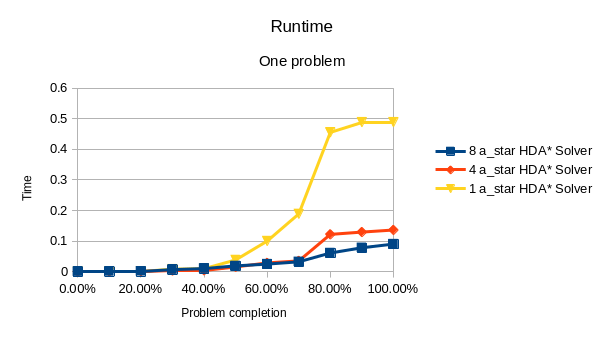
\includegraphics[width=\textwidth]{Media/Ch2/Runtime_One_Problem_Linear.png}
    \caption{Tiempo de ejecución de un único problema.}
    \label{fig:Runtime_One_Problem_Linear}
\end{figure}

Como se puede ver, el diagrama es de poca utilidad debido a la
complejidad del problema.
Para poder observar con mejor los resultados,
se utiliza un eje vertical con una escala logarítmica
(figura \ref{fig:Runtime_One_Problem_Log}).

\begin{figure}[h]
    \centering
    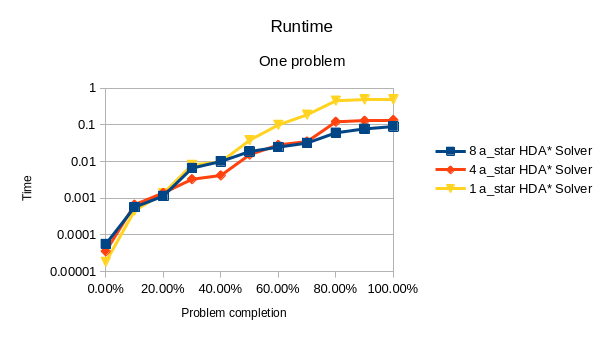
\includegraphics[width=\textwidth]{Media/Ch2/Runtime_One_Problem_Log.png}
    \caption{Tiempo de ejecución de un único problema (escala logarítmica).}
    \label{fig:Runtime_One_Problem_Log}
\end{figure}

Estas observaciones verifican que la complejidad del problema
a resolver es cuadrática, como era de esperar.

\begin{notebox}
    Esta sección contiene diversas gráficas de las métricas obtenidas,
    obsérvese con detalle la escala utilizada en el eje de ordenadas de cada una
    ya que en algunos casos será logarítmica.
\end{notebox}

\subsection{Comparativa de heurísticos}
\index{Resultados!Heurísticos}

Como ya se discutió en la sección sobre optimización (\ref{ssec:Heuristicos}),
existen varias implementaciones de la función heurística que da al algoritmo
A* su particular comportamiento de ir `dirigido' hacia la solución.
En esta investigación se han implementado dos heurísticos:
uno de ellos busca una solución que se acerque a la óptima lo máximo posible
mientras que el otro busca la solución priorizando la velocidad del algoritmo.
A continuación se comparan los heurísticos utilizando la implementación paralela HDA*.

En primer lugar se observa que existe un limitado número de soluciones
propuestas, las más comunes siendo también las más bajas: 452 y 472.
Respecto al tiempo de ejecución, las pruebas que utilizan el heurístico rápido
reducen el tiempo de ejecución en varias magnitudes.

\begin{figure}[h]
    \begin{subfigure}{.5\textwidth}
        \begin{center}
            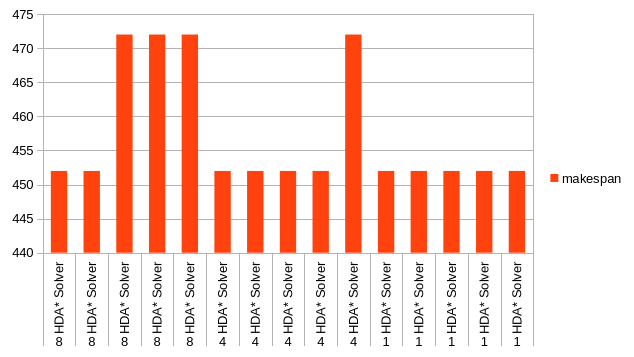
\includegraphics[width=\textwidth]{Media/Ch2/Makespan_Slow_HDA.png}
            \subcaption{\italic{Makespan} del heurístico lento.}
        \end{center}
    \end{subfigure}
    \begin{subfigure}{.5\textwidth}
        \begin{center}
            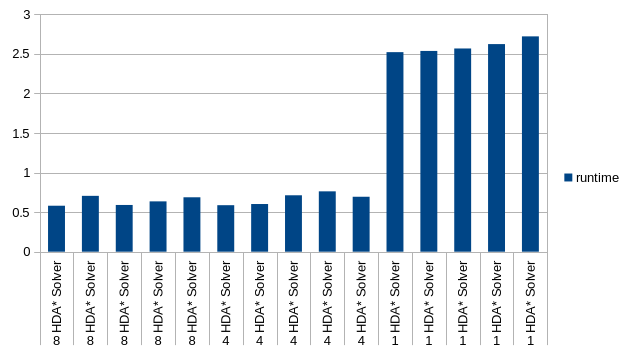
\includegraphics[width=\textwidth]{Media/Ch2/Runtime_Slow_HDA.png}
            \subcaption{Tiempo de ejecución del heurístico lento.}
        \end{center}
    \end{subfigure}
    \caption{Métricas heurístico lento.}
    \label{fig:HeuristicoLento}
\end{figure}

\begin{figure}[h]
    \begin{subfigure}{.5\textwidth}
        \begin{center}
            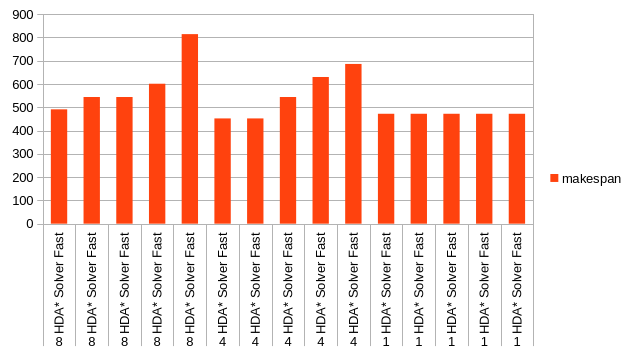
\includegraphics[width=\textwidth]{Media/Ch2/Makespan_Fast_HDA.png}
            \subcaption{\italic{Makespan} del heurístico rápido.}
        \end{center}
    \end{subfigure}
    \begin{subfigure}{.5\textwidth}
        \begin{center}
            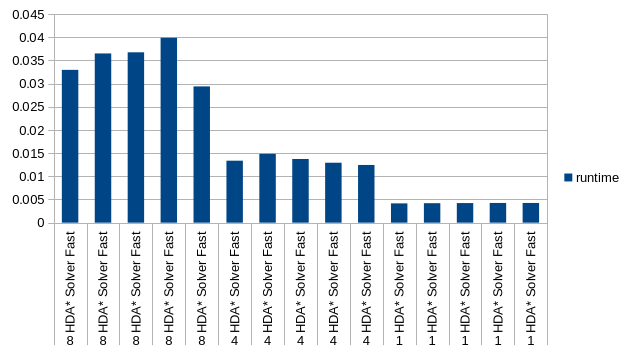
\includegraphics[width=\textwidth]{Media/Ch2/Runtime_Fast_HDA.png}
            \subcaption{Tiempo de ejecución del heurístico rápido.}
        \end{center}
    \end{subfigure}
    \caption{Métricas heurístico rápido.}
    \label{fig:HeuristicoRapido}
\end{figure}

Analizandolas por separado, las ejecuciones que utilizan el heurístico lento
retornaron siempre 452 o 472, los dos mejores resultados y se vieron
beneficiadas por el uso de varios hilos.
Por otro lado, las ejecuciones que utilizan el heurístico rápido
sólo retornaron 452 o 472 en algunas instancias y no se vieron
beneficiadas por el uso de varios hilos
(Véase figuras \ref{fig:HeuristicoLento} y \ref{fig:HeuristicoRapido}).

Sería razonable suponer que el heurístico rápido
sí se vería beneficiado por el paralelismo si el tamaño del
problema fuese lo suficientemente grande.
Para comprobar esta hipótesis, se ha creado un conjunto
con un tamaño mucho mayor (70x10) y se ha obtenido el \italic{speedup}.

\begin{figure}[h]
    \centering
    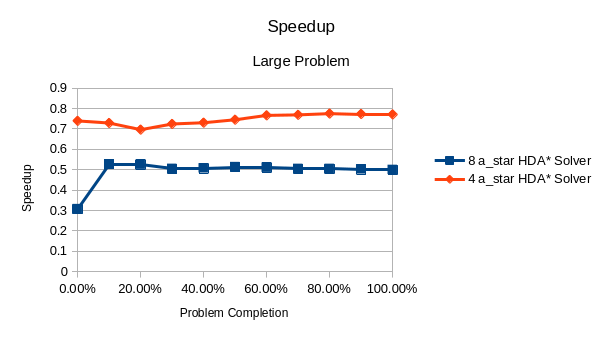
\includegraphics[width=\textwidth]{Media/Ch2/Speedup_Large_Problem.png}
    \caption{\italic{Speedup} en un problema de gran tamaño.}
    \label{fig:Speedup_Large_Problem}
\end{figure}

La gráfica (\ref{fig:Speedup_Large_Problem}) muestra que incluso en un problema de mayor tamaño
la versión monohilo es más rápida que las multihilo.
Esta investigación no ha podido encontrar un conjunto de datos
en el que utilizando el heurístico rápido valga la pena el paralelismo.
No obstante, se ha observado que a medida que el tamaño
del problema incrementa, el \italic{speedup} también se ve incrementando
por lo que si se supone que la tendencia del \italic{speedup}
se mantiene, sería razonable suponer que existe un tamaño de
problema donde sí vale la pena utilizar varios hilos y 
el heurístico rápido.

\subsection{Cuellos de botella en secciones críticas}
\index{Resultados!Cuellos de botella}

Los algoritmos que utilizan estructuras de datos compartidas
para almacenar los nodos y sus costes se ven gravemente
afectadas cuando el tamaño de estas estructuras incrementa.
Como esta información es compartida por todos los hilos,
es necesario acceder a ella de forma serializada,
reduciendo notablemente el \italic{speedup}.

En algunos casos extremos es posible incluso
que versiones monohilo del mismo algoritmo
tengan mejor rendimiento que versiones paralelas.
Nótese que el \italic{speedup} del algoritmo FCFS
cuando se utilizan varios hilos (respecto a un hilo solo)
es inferior a $1$.
(Véase figura \ref{fig:ParalelismoFCFS}).

\begin{figure}[h]
    \begin{subfigure}{.5\textwidth}
        \begin{center}
            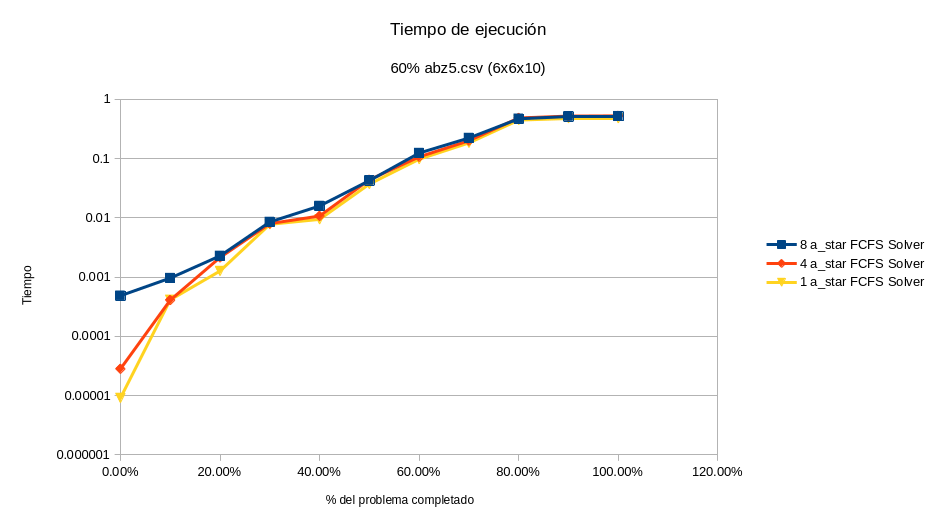
\includegraphics[width=\textwidth]{Media/Ch2/Runtime_FCFS_Log.png}
            \subcaption{Tiempo de ejecución de FCFS.}
        \end{center}
    \end{subfigure}
    \begin{subfigure}{.5\textwidth}
        \begin{center}
            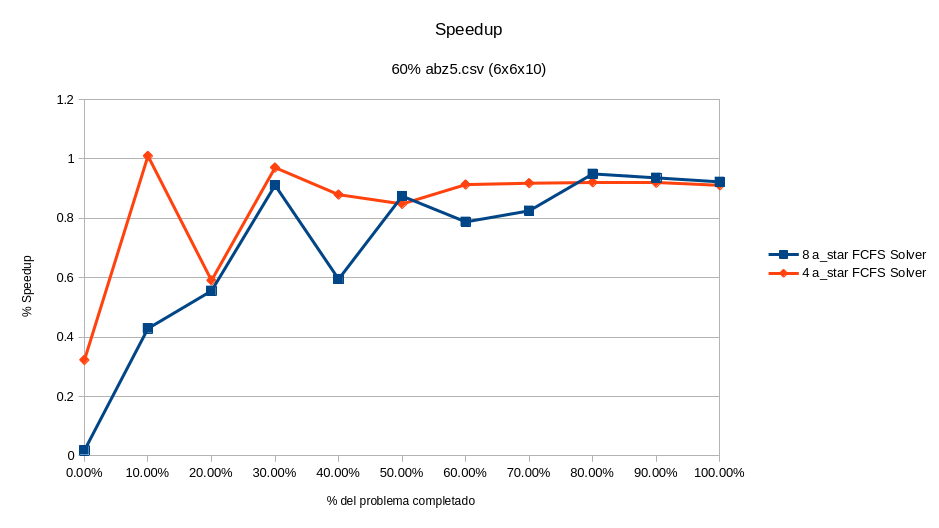
\includegraphics[width=\textwidth]{Media/Ch2/Speedup_FCFS.png}
            \subcaption{\italic{Speedup} de FCFS.}
        \end{center}
    \end{subfigure}
    \caption{Métricas de paralelismo en FCFS.}
    \label{fig:ParalelismoFCFS}
\end{figure}

Por otro lado, algoritmos como el HDA*
que utilizan una estructura de datos privada para cada hilo
no ven sus tareas serializadas,
incrementando notablemente el \italic{speedup}
(Véase figura \ref{fig:ParalelismoHDA}).

\begin{figure}[h]
    \begin{center}
        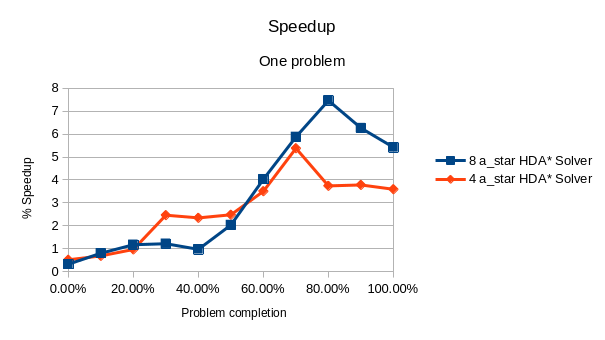
\includegraphics[width=\textwidth]{Media/Ch2/Speedup_One_Problem.png}
    \end{center}
    \caption{\italic{Speedup} de HDA*.}
    \label{fig:ParalelismoHDA}
\end{figure}

Nótese que al inicio del problema (aproximadamente hasta completar el $30\percentsign$)
la versión monohilo de los algoritmos es más rápida que cualquier multihilo.
Esto se debe a que para tamaños de problema muy pequeños
el coste de crear $N$ hilos es superior al de resolver el problema
utilizando uno sólo.

Si se observa el \italic{speedup} al final del problema,
la versión con cuatro hilos tiene un \italic{speedup}
de $3.5$ mientras que la de ocho tiene $5.5$.
Esto implica que al utilizar cuatro hilos,
el algoritmo ha sido capaz de aprovecharlos casi al máximo
ya que el tiempo de ejecución casi se reduce en 4
veces.
Mientras tanto, al utilizar 8 hilos el algoritmo
no ha sido capaz de rentabilizarlos en la misma proporción.
Este déficit podría deberse a que el tamaño del problema
es demasiado pequeño para aprovechar la cantidad de hilos
o podría deberse al propio diseño del algoritmo.

\subsection{Comparativa de algoritmos}
\index{Resultados!Comparativa de algoritmos}

Como es de esperar, el rendimiento monohilo de todas
las implementaciones es el mismo.
Todas las implementaciones están diseñadas de forma
que al ser ejecutadas con un sólo hilo
el algoritmo sea el A* básico.

\begin{figure}[h]
    \begin{center}
        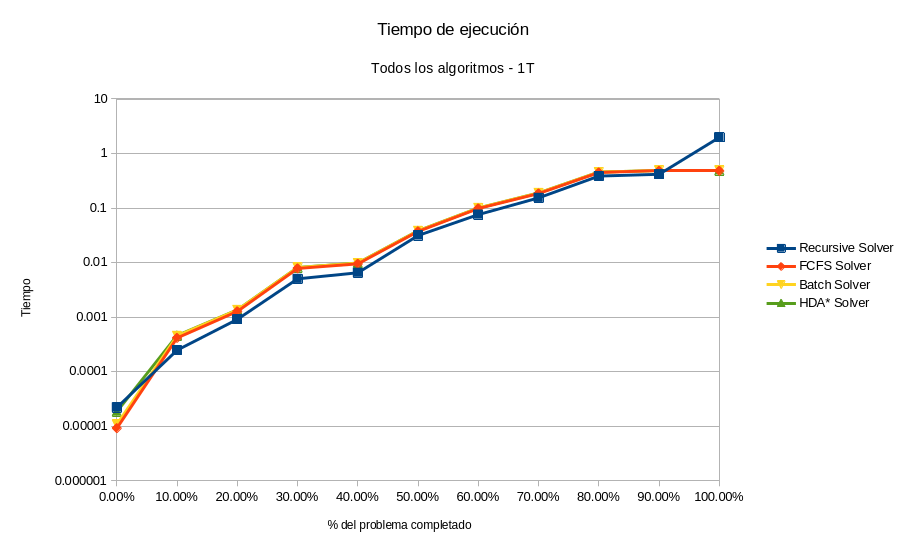
\includegraphics[width=\textwidth]{Media/Ch2/Runtime_All_Algorithms_1.png}
    \end{center}
    \caption{Tiempo de ejecución de todos los algoritmos (1 hilo).}
    \label{fig:MetricasSinglethread}
\end{figure}

\begin{figure}[h]
    \begin{subfigure}{.5\textwidth}
        \begin{center}
            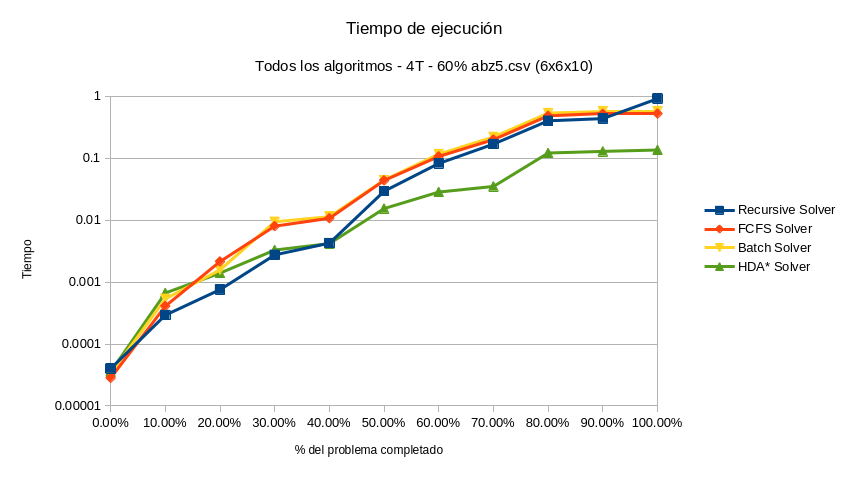
\includegraphics[width=\textwidth]{Media/Ch2/Runtime_All_Algorithms_4.png}
            \subcaption{Tiempo de ejecución de todos los algoritmos (4 hilos).}
        \end{center}
    \end{subfigure}
    \begin{subfigure}{.5\textwidth}
        \begin{center}
            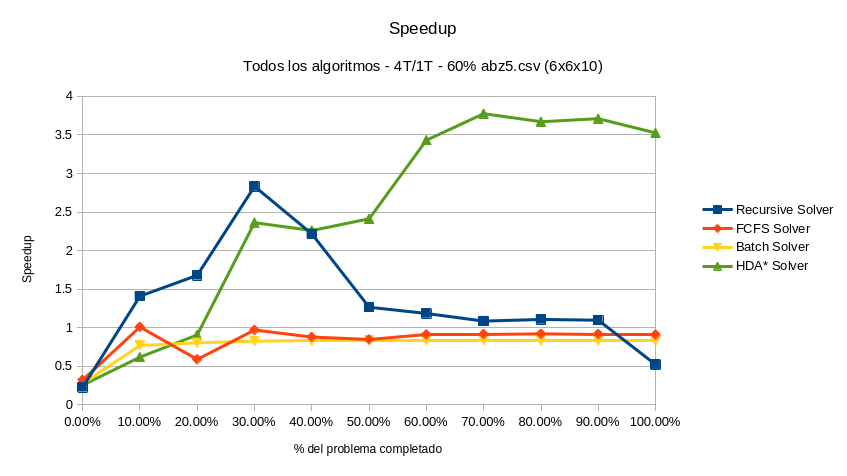
\includegraphics[width=\textwidth]{Media/Ch2/Speedup_All_Algorithms_4.png}
            \subcaption{\italic{Speedup} de todos los algoritmos (4 hilos).}
        \end{center}
    \end{subfigure}
    \caption{Métricas con 4 hilos.}
    \label{fig:Metricas4Thread}
\end{figure}

Al utilizar cuatro hilos (figura \ref{fig:Metricas4Thread}), se puede comenzar a ver una diferencia clara
en el rendimiento del algoritmo HDA*, que obtiene un \italic{speedup}
de casi 4.

\begin{figure}[h]
    \begin{subfigure}{.5\textwidth}
        \begin{center}
            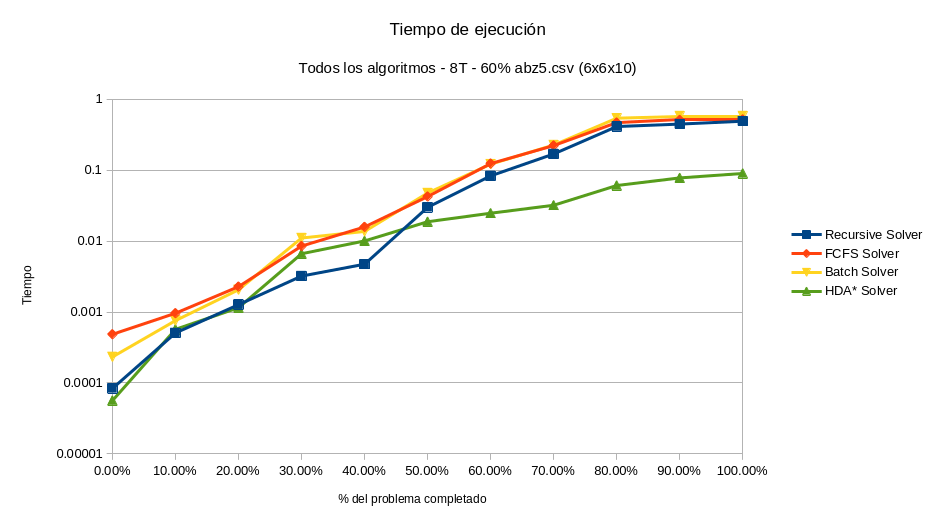
\includegraphics[width=\textwidth]{Media/Ch2/Runtime_All_Algorithms_8.png}
            \subcaption{Tiempo de ejecución de todos los algoritmos (8 hilos).}
        \end{center}
    \end{subfigure}
    \begin{subfigure}{.5\textwidth}
        \begin{center}
            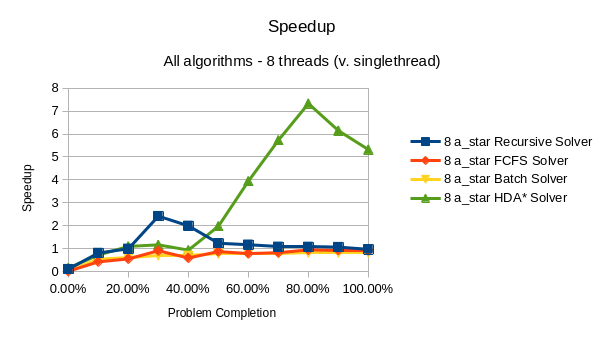
\includegraphics[width=\textwidth]{Media/Ch2/Speedup_All_Algorithms_8.png}
            \subcaption{\italic{Speedup} de todos los algoritmos (8 hilos).}
        \end{center}
    \end{subfigure}
    \caption{Métricas con 8 hilos.}
    \label{fig:Metricas8Thread}
\end{figure}

Al utilizar ocho hilos (figura \ref{fig:Metricas8Thread}), el algoritmo HDA* incremente aún más su diferencia
en el tiempo de ejecución con respecto al resto de algoritmos,
aunque esta vez el \italic{speedup} fluctua más.
De cualquier forma, parece ser capaz de alcanzar casi 8.

La principal conclusión de estas observaciones es que
(al menos en los conjuntos de datos observados)
el paralelismo es sólo rentable si se implementa el HDA*.
En el resto de casos, el paralelismo sólo sirve para
gastar núcleos y ciclos de CPU a cambio de nada.

\pagebreak

\subsection{Casos particulares}
\index{Resultados!Casos particulares}

Vistos los resultados anteriores
se podrían dar como obsoletas algunas de las versiones
paralelas por ofrecer muy pocas mejoras frente a otras
versiones monohilo.
No obstante, existen casos particulares del problema
donde estas versiones fácilmente descartables
podrían presentar una solución mucho más interesante.

Estos casos particulares generalmente involucran
la posibilidad de que la población de nodos sea
repartida entre los diferentes hilos de forma
que cada uno tenga una sección parcial o totalmente
independiente del resto.
A continuación se presentan algunos de estos casos.

\subsubsection{Varios estados iniciales}
\index{Resultados!Casos particulares!Varios estados iniciales}

Si el problema a resolver tiene varios estados iniciales
sería posible asignar cada estado a un hilo (o grupo de hilos)
de forma que cada uno busque una solución desde su estado inicial.

\subsubsection{Estados solución intermedios}
\index{Resultados!Casos particulares!Estados solución intermedios}

Si se conoce algún nodo intermedio de la solución
sería posible dividir el problema en dos,
de forma que un hilo resuelva una de las partes
\footnote{Si existiese más de un nodo intermedio conocido,
el problema se podría seguir subdividiendo entre más hilos.}.
Por ejemplo, si del problema se conocen el nodo inicial $A$,
el final $E$ y los intermedios $B$, $C$ y $D$,
la solución se podría obtener repartiendo el
trabajo entre 4 hilos diferentes:
\begin{enumerate}[start=0, itemsep=0.25px]
    \item Hilo 0: Resolver camino desde nodo $A$ hasta $B$.
    \item Hilo 1: Resolver camino desde nodo $B$ hasta $C$.
    \item Hilo 2: Resolver camino desde nodo $C$ hasta $D$.
    \item Hilo 3: Resolver camino desde nodo $D$ hasta $E$.
\end{enumerate}
